\section{Experimental Results}
\label{sec:experimentalResults}

A first prototype was build using the specifications described in section \ref{sec:TechnicalApproach}. Using this prototype initial tests of the COAM drive and the resulting laser scanning procedure were conducted. In this section an overview over the results will be given.

\subsection{3D Laser Scanning}
\label{sec:experimentalResults:3DLaserScanning}

The test of the 3D Laser Scanning was carried out in 3 phases. First a semi stationary scan, moving the robot manually in a limited manner (tilting it by approximately $\SI{45}{\degree}$) without its exterior shell, was performed. This resulted in the point cloud in figure \ref{sec:experimentalResults:3DLaserScanning:fig:firstpointcloud}. For the second test the same movement was used. However, this time the outside shell of the robot  was present. This resulted in figure \ref{sec:experimentalResults:3DLaserScanning:fig:secondpointcloud}. Finally a test of the overall system was conducted using the COAM-drive as motor resulting in multiple revolutions. The point cloud can be seen in figure \ref{sec:experimentalResults:3DLaserScanning:fig:thirdpointcloud}.

\begin{figure}
\centering
\begin{subfigure}[b]{0.49\textwidth}
	\centering
	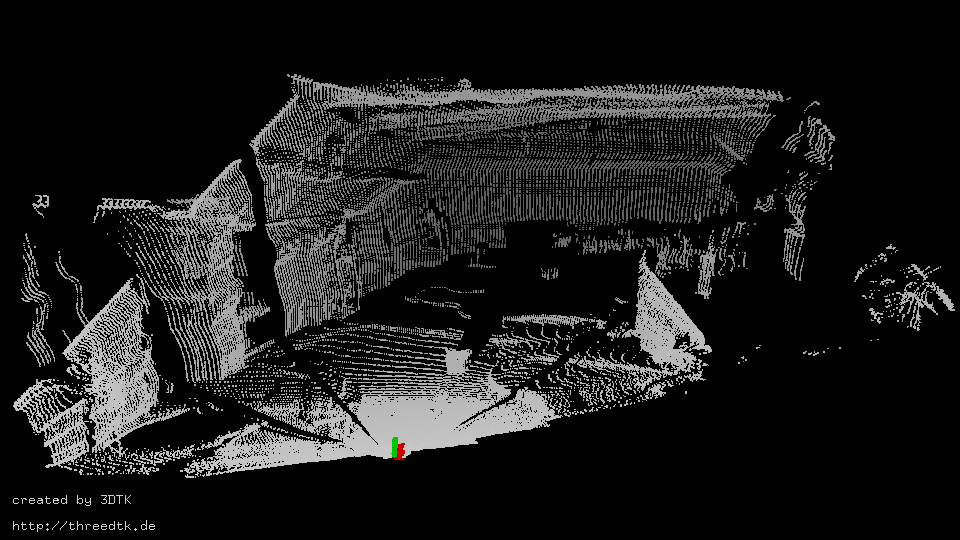
\includegraphics[width=\textwidth,trim={0 1cm 0 1cm},clip]{../Media/FirstDecentMap}
	\caption{Test with limited movement and no exterior shell.}
	\label{sec:experimentalResults:3DLaserScanning:fig:firstpointcloud}
\end{subfigure}
\hfill
\begin{subfigure}[b]{0.49\textwidth}
	\centering
	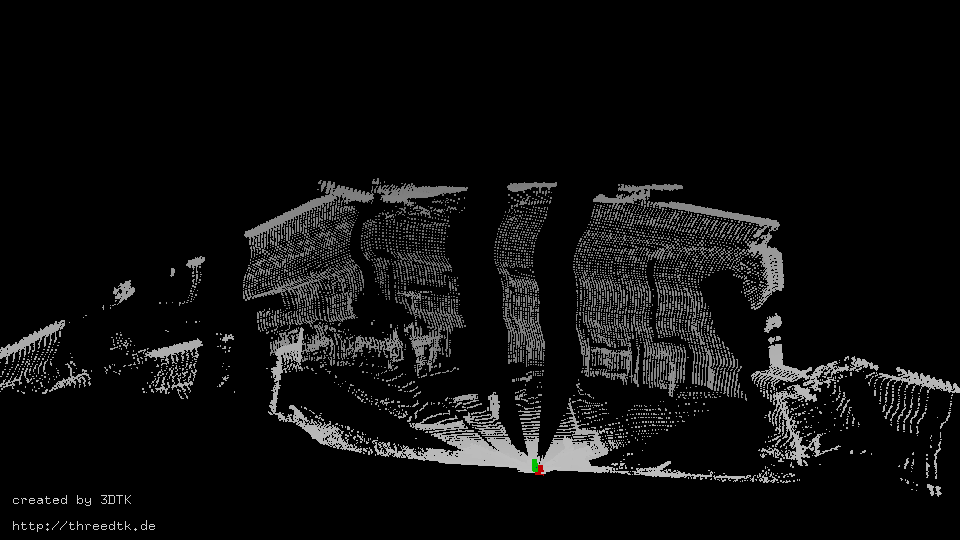
\includegraphics[width=\textwidth,trim={0 1cm 0 1cm},clip]{../Media/testScanWithTop}
	\caption{Test with limited movement but present exterior shell.}
	\label{sec:experimentalResults:3DLaserScanning:fig:secondpointcloud}
\end{subfigure}
\\
\begin{subfigure}[b]{\textwidth}
	\centering
	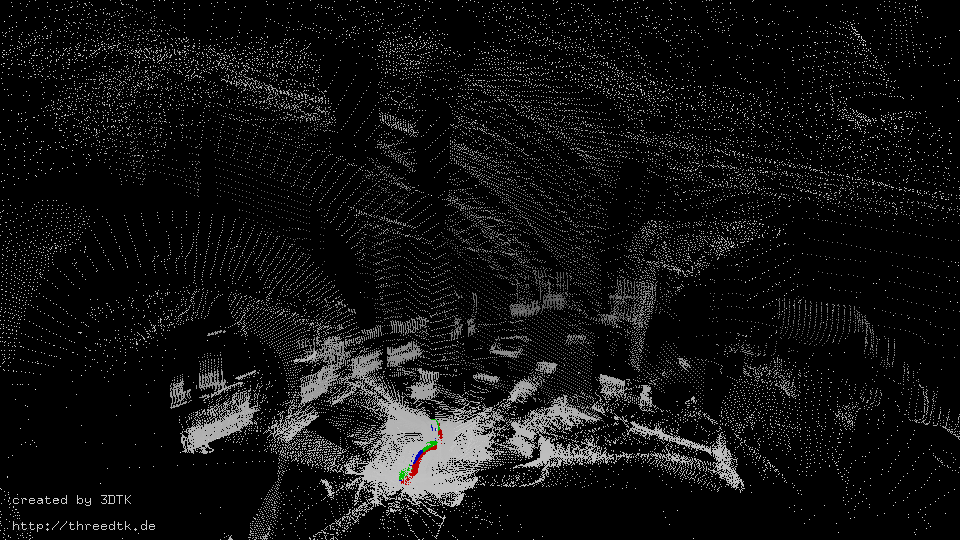
\includegraphics[width=\textwidth,trim={0 1cm 0 1cm},clip]{../Media/RollingTestMap}
	\caption{Test with exterior shell and full movement (i.e. multiple revolutions).}
	\label{sec:experimentalResults:3DLaserScanning:fig:thirdpointcloud}
\end{subfigure}
\caption{3D Point cloud results of different test scenarios of the system.}
\end{figure}

The clearest point cloud was obtained from the first test (figure \ref{sec:experimentalResults:3DLaserScanning:fig:firstpointcloud}). This can be contributed to the fact, that in this test the exterior shell was missing. Usually it is partially reflecting the beams of the laser scanner. Thus, the laser scanner is measuring the shell instead of the environment around it. When looking at figure \ref{sec:experimentalResults:3DLaserScanning:fig:secondpointcloud} we can see certain lines being blocked that weren't in the previous test further showing the reflection of the laser beams by the shell. This effect is amplified as soon as the robot starts rolling. Specifically this is manifested in a large number of measurement points along the path of the robot (figure \ref{sec:experimentalResults:3DLaserScanning:fig:thirdpointcloud}).

Furthermore, the asynchrony of the pose determination sub-system and the laser scanner adds to the messiness of the point-cloud. Specifically this can be seen in figure \ref{sec:experimentalResults:3DLaserScanning:fig:thirdpointcloud} as there are points detected underneath the surface the robot was rolling on. 

\subsection{COAM Drive}
\label{sec:experimentalResults:COAMDrive}

The drive based on conversation of angular momentum was able to accelerate the L.U.N.A. sphere reliably. The angular acceleration of the whole sphere measured by the IMU - system in one test run can be seen in figure \ref{sec:experimentalResults:COAMDrive:fig:angvel}. It can be seen that the acceleration along the rotational axis of the flywheels rises while the accelerations along the other axes remain lower, albeit are noisy. The accelerations along the other axis can mostly be contributed to vibrations and some tilt of the robot. The vibrations are results of inexact drilling of the flywheels such that there is an imbalance. At the main test site the ground was a hard, slippery concrete floor. In such a scenario the vibrations add up and lead to slippage such that the robot no longer rolls. However, when tested on a rubber surface (a running track) the vibrations are absorbed, such that the acceleration process happens reliably.

\begin{figure}
\centering
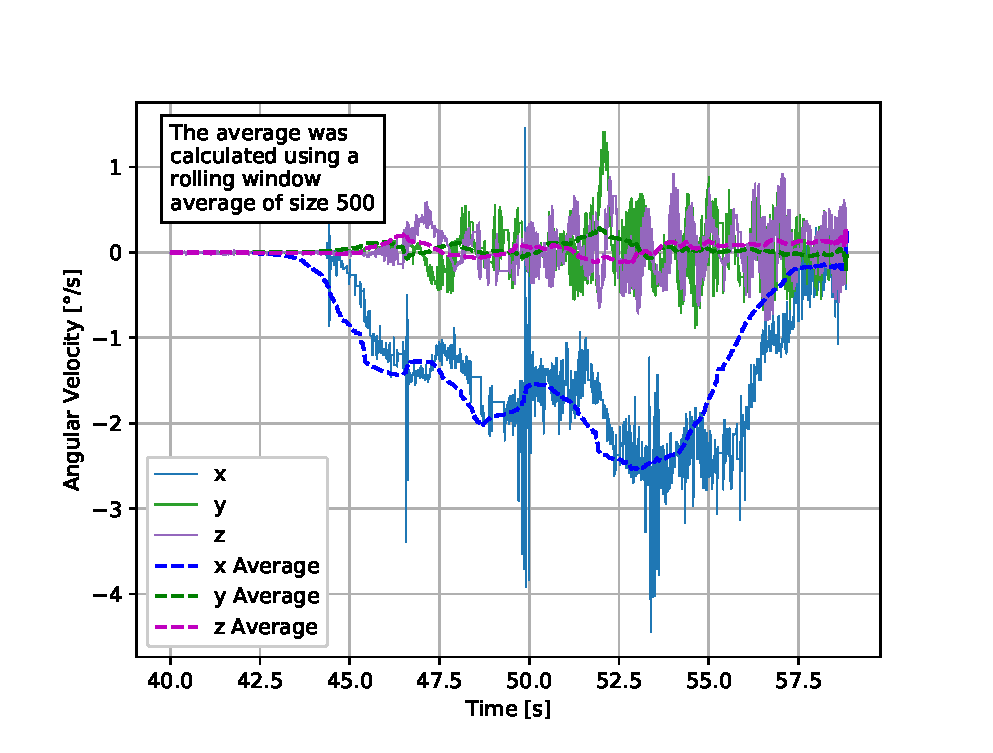
\includegraphics[width=\textwidth]{./plotsAndScripts/angVel-2020-01-29-16-14-54/ang-vel}
\caption{Angular velocities of the L.U.N.A. - sphere during a test run. The flywheels rotate around the x-axis in positive direction. Velocities in the other direction can mostly be contributed to vibrations and tilt of the robot.}
\label{sec:experimentalResults:COAMDrive:fig:angvel}
\end{figure}